\chapter{METHODOLOGY}
\begin{normaltext}
This project aims to fine-tune Llama-2 7B large language model for Python code generation. 
The methodology is structured in three phases: dataset preparation, fine-tuning, and evaluation. 
Figure~\ref{fig:finalmodel} shows the final model after fine-tuning where Figure \ref{fig:decoder} represents the decoder block diagram with QLoRA adapter.

\vspace{10pt}
\begin{figure}[H]
    \centering
    \includegraphics[width=0.65\linewidth]{model.jpg}
    \caption{System Block Diagram}
    \label{fig:finalmodel}
\end{figure}

\begin{figure}[H]
    \centering
    \includegraphics[width=0.85\linewidth]{decoder.jpg}
    \caption{Decoder Block Diagram with QLoRA Adapter}
    \label{fig:decoder}
\end{figure}

The final model is a Decoder-only Transformer architecture enhanced with QLoRA for memory-efficient fine-tuning. The process begins with raw text being converted into Input Embeddings and combined with Positional Encoding to help the model understand the order of words. This combined vector enters a stack of 31 identical Decoder Layers. Each layer follows a specific sequence: the data is first normalized via RMSNorm before entering the Self-Attention block, where the model weighs the importance of different words in the context. Crucially, the QLoRA Adapter  is injected here, allowing the model to learn task-specific updates through small, trainable matrices while keeping the massive original weights frozen and quantized.After the attention phase, the signal is normalized again and passed into the FFN, which also features a QLoRA adapter injection to refine the model's high-level reasoning. These "adapter" paths are added back to the main data flow using residual connections, ensuring the model retains its base knowledge while incorporating new fine-tuned patterns. Once the data exits the final decoder layer, it passes through a Linear layer to project it back into the vocabulary size and a Softmax function to produce Probabilities. These probabilities represent the model's prediction for the most likely next word in the sequence, which is then fed back into the system to generate text auto-regressively.

\vspace{18pt}
% ---------------------------------------------------------
\section{Dataset Description and Preparation}

Fine-tuning Llama-2 7B for Python code generation requires a high-quality, domain-specific dataset 
containing diverse programming tasks and their corresponding solutions. 
We will construct a composite dataset from multiple reputable open-source sources.
\end{normaltext}
\subsection{Dataset Sources and Composition}
\begin{normaltext}

\begin{table}[H]
    \centering
    \caption{Dataset Sources and Composition}
    \begin{tabularx}{\textwidth}{|>{\bfseries}p{1.8cm}|>{\raggedright\arraybackslash}X|>{\raggedright\arraybackslash}X|>{\raggedright\arraybackslash}p{1.5cm}|}
        \hline
        \textbf{Dataset} & \textbf{Size} & \textbf{Content \& Reason} & \textbf{License} \\
        \hline
        FlyTech Python Code Dataset (2025) & $\sim$42,000 pairs & Python scripts with comments, docstrings, and structured tasks. Curated for code generation with high-quality, well-commented code and diverse algorithmic/real-world examples. & MIT License \\
        \hline
        Python Code Instructions 18k (Alpaca-style) & $\sim$18,000 pairs & Instruction prompts and Python responses. Matches instruction-tuning structure; provides human-readable prompts and increases prompt diversity. & CC BY-NC 4.0 \\
        \hline
        LeetCode Programming Problems (Evaluation Only) & $\sim$200--300 problems & Problem descriptions and reference solutions. Provides competitive programming tasks and enables functional correctness testing. & Fair use \\
        \hline
    \end{tabularx}
    
    \label{tbl:datasets}
\end{table}

We will standardize the problem set used from LeetCode/HackerRank and not directly extract their internal datasets.  
\end{normaltext}


\subsection{Dataset Processing Pipeline}
\begin{normaltext}
    The collected dataset will undergo several preprocessing steps to ensure quality and consistency before training:
    \begin{itemize}
        \item Duplicate removal
        All repeated or identical instruction–code pairs will be removed to eliminate redundancy and reduce overfitting.

        \item Filtering Incomplete Python Code
        Examples containing syntactically incorrect or incomplete Python code will be discarded using rule-based checks and code-parsing techniques.
        \item Adding Chain-of-Thought (CoT) Explanations
        Each example will be enriched with a brief chain-of-thought explanation describing the reasoning steps used to solve the instruction.This helps the model learn structured reasoning patterns.
        \item Normalization and Formatting
        All samples will be standardized with consistent indentation, spacing, variable naming, and overall formatting.
    \end{itemize}
    \textbf{Final Dataset Size (Expected)}
  
     
        \begin{table}[h]
               \begin{center}
        \caption{Final Dataset Size (Expected)}
        \begin{tabular}{l r}
        \textbf{Dataset} & \textbf{Count} \\
        \hline
        FlyTech & $\sim$40,000 \\
        Alpaca & $\sim$17,000 \\
        \hline
        Total usable examples & $\sim$57,000 \\
        \end{tabular}
         \end{center}
        \end{table}
       
    
\end{normaltext}


\subsection{Train/Validation Split}
\begin{normaltext}
The cleaned dataset is partitioned into three subsets to support effective model training and evaluation. Specifically, 90\% of the data is allocated for training, providing the model with sufficient examples to learn underlying patterns. Another 5\% is used as a validation set to monitor overfitting during training. The remaining 5\% forms the evaluation set, which is kept strictly separate and consists of data from platforms such as LeetCode and HackerRank to ensure an unbiased assessment of the model’s generalization capability. The evaluation set (LeetCode/HackerRank) remains entirely separate.
\end{normaltext}


\subsection{Instruction Formatting and Tokenization}
\begin{normaltext}
    Each training example will be converted into an instruction-style structure.

    \begin{quote}
    \begin{ttfamily}
    Instruction Write a Python code for printing whether a given number is Armstrong.
    
    Chain of thought:
    An Armstrong number is a number that is equal to the sum of its own digits each raised to the power of the number of digits.
    To check if a number is an Armstrong number, we can follow these steps:
    \\1. Convert the number to a string to easily iterate over each digit.
    \\2. Calculate the number of digits in the number.
    \\3. For each digit, raise it to the power of the number of digits and sum these values.
    \\4. Compare the sum to the original number. If they are equal, then it is an Armstrong number; otherwise, it is not.
    
    Response
    \begin{verbatim}
    num = int(input("Enter a number "))
    digits = len(str(num))
    armstrong_sum = sum(int(d)**digits for d in str(num))
    if num == armstrong_sum:
        print(f"{num} is an Armstrong number")
    else:
        print(f"{num} is not an Armstrong number")
    \end{verbatim}
    \end{ttfamily}
    \end{quote}

    Finally, all training examples will be tokenized using the Llama tokenizer to ensure full compatibility with the pretrained Llama-2 7B model.This guarantees that special tokens, vocabulary indices, and formatting structures align correctly during QLoRA fine-tuning, preventing token-mismatch issues and maintaining optimal model performance.

\end{normaltext}

% ---------------------------------------------------------
\section{Model Fine-Tuning}
\begin{normaltext}
We will fine-tune the Llama 2 model using QLoRA to enable efficient Python code generation from textual prompts. 
The base model will be loaded with pretrained and 4-bit quantized weights to reduce memory usage.
\end{normaltext}

\subsection{Fine-Tuning Approach}
\begin{normaltext}
Fine-tuning follows the instruction-tuning paradigm given a prompt x, the model predicts the next token in the target Python code sequence y. Mathematically, the model maximizes the likelihood of the entire sequence consisting of instruction, reasoning, and output as shown in \ref{eq:loss}.


\begin{equation}\label{eq:loss}
\text{loss} = -\sum_{t=1}^{T} \log P_{\theta} (y_{t}^{\text{true}} \mid y_{<t}, x)
\end{equation}

Model parameters are updated using gradient descent

\begin{equation}
\theta_{i+1} \leftarrow \theta_i - \alpha \frac{\partial (\text{loss})}{\partial \theta}
\end{equation}


To improve reasoning quality and reduce hallucination, we additionally include Chain-of-Thought (CoT) annotations inside the training samples. Each training example consists of Instruction Human-written reasoning (CoT) Final code output. This encourages the model to learn step-by-step reasoning patterns before producing the final answer. The CoT component explicitly teaches the model how to plan the solution how to reason before generating code. This approach is known to significantly reduce hallucinations and improve generalization in small models.

% ---------------------------------------------------------
\vspace{18 pt}
\subsection{QLoRA for Efficient Training}

QLoRA enables parameter-efficient fine-tuning by
\begin{itemize}
    \item Keeping the pretrained model weights frozen
    \item Loading weights in 4-bit quantization
    \item Adding trainable low-rank adapter matrices inside transformer blocks
\end{itemize}
% \begin{figure}[h]
%     \centering
%     \includegraphics[width=0.85\linewidth]{without_qlora.png} % Uncomment when you add the figure
%     \caption{Base Model Finetuning with out QLoRA Adapter Layers}
%     \label{figBase Model Finetuning with out QLoRA Adapter Layer}
% \end{figure}

\begin{figure}[H]
    \centering
    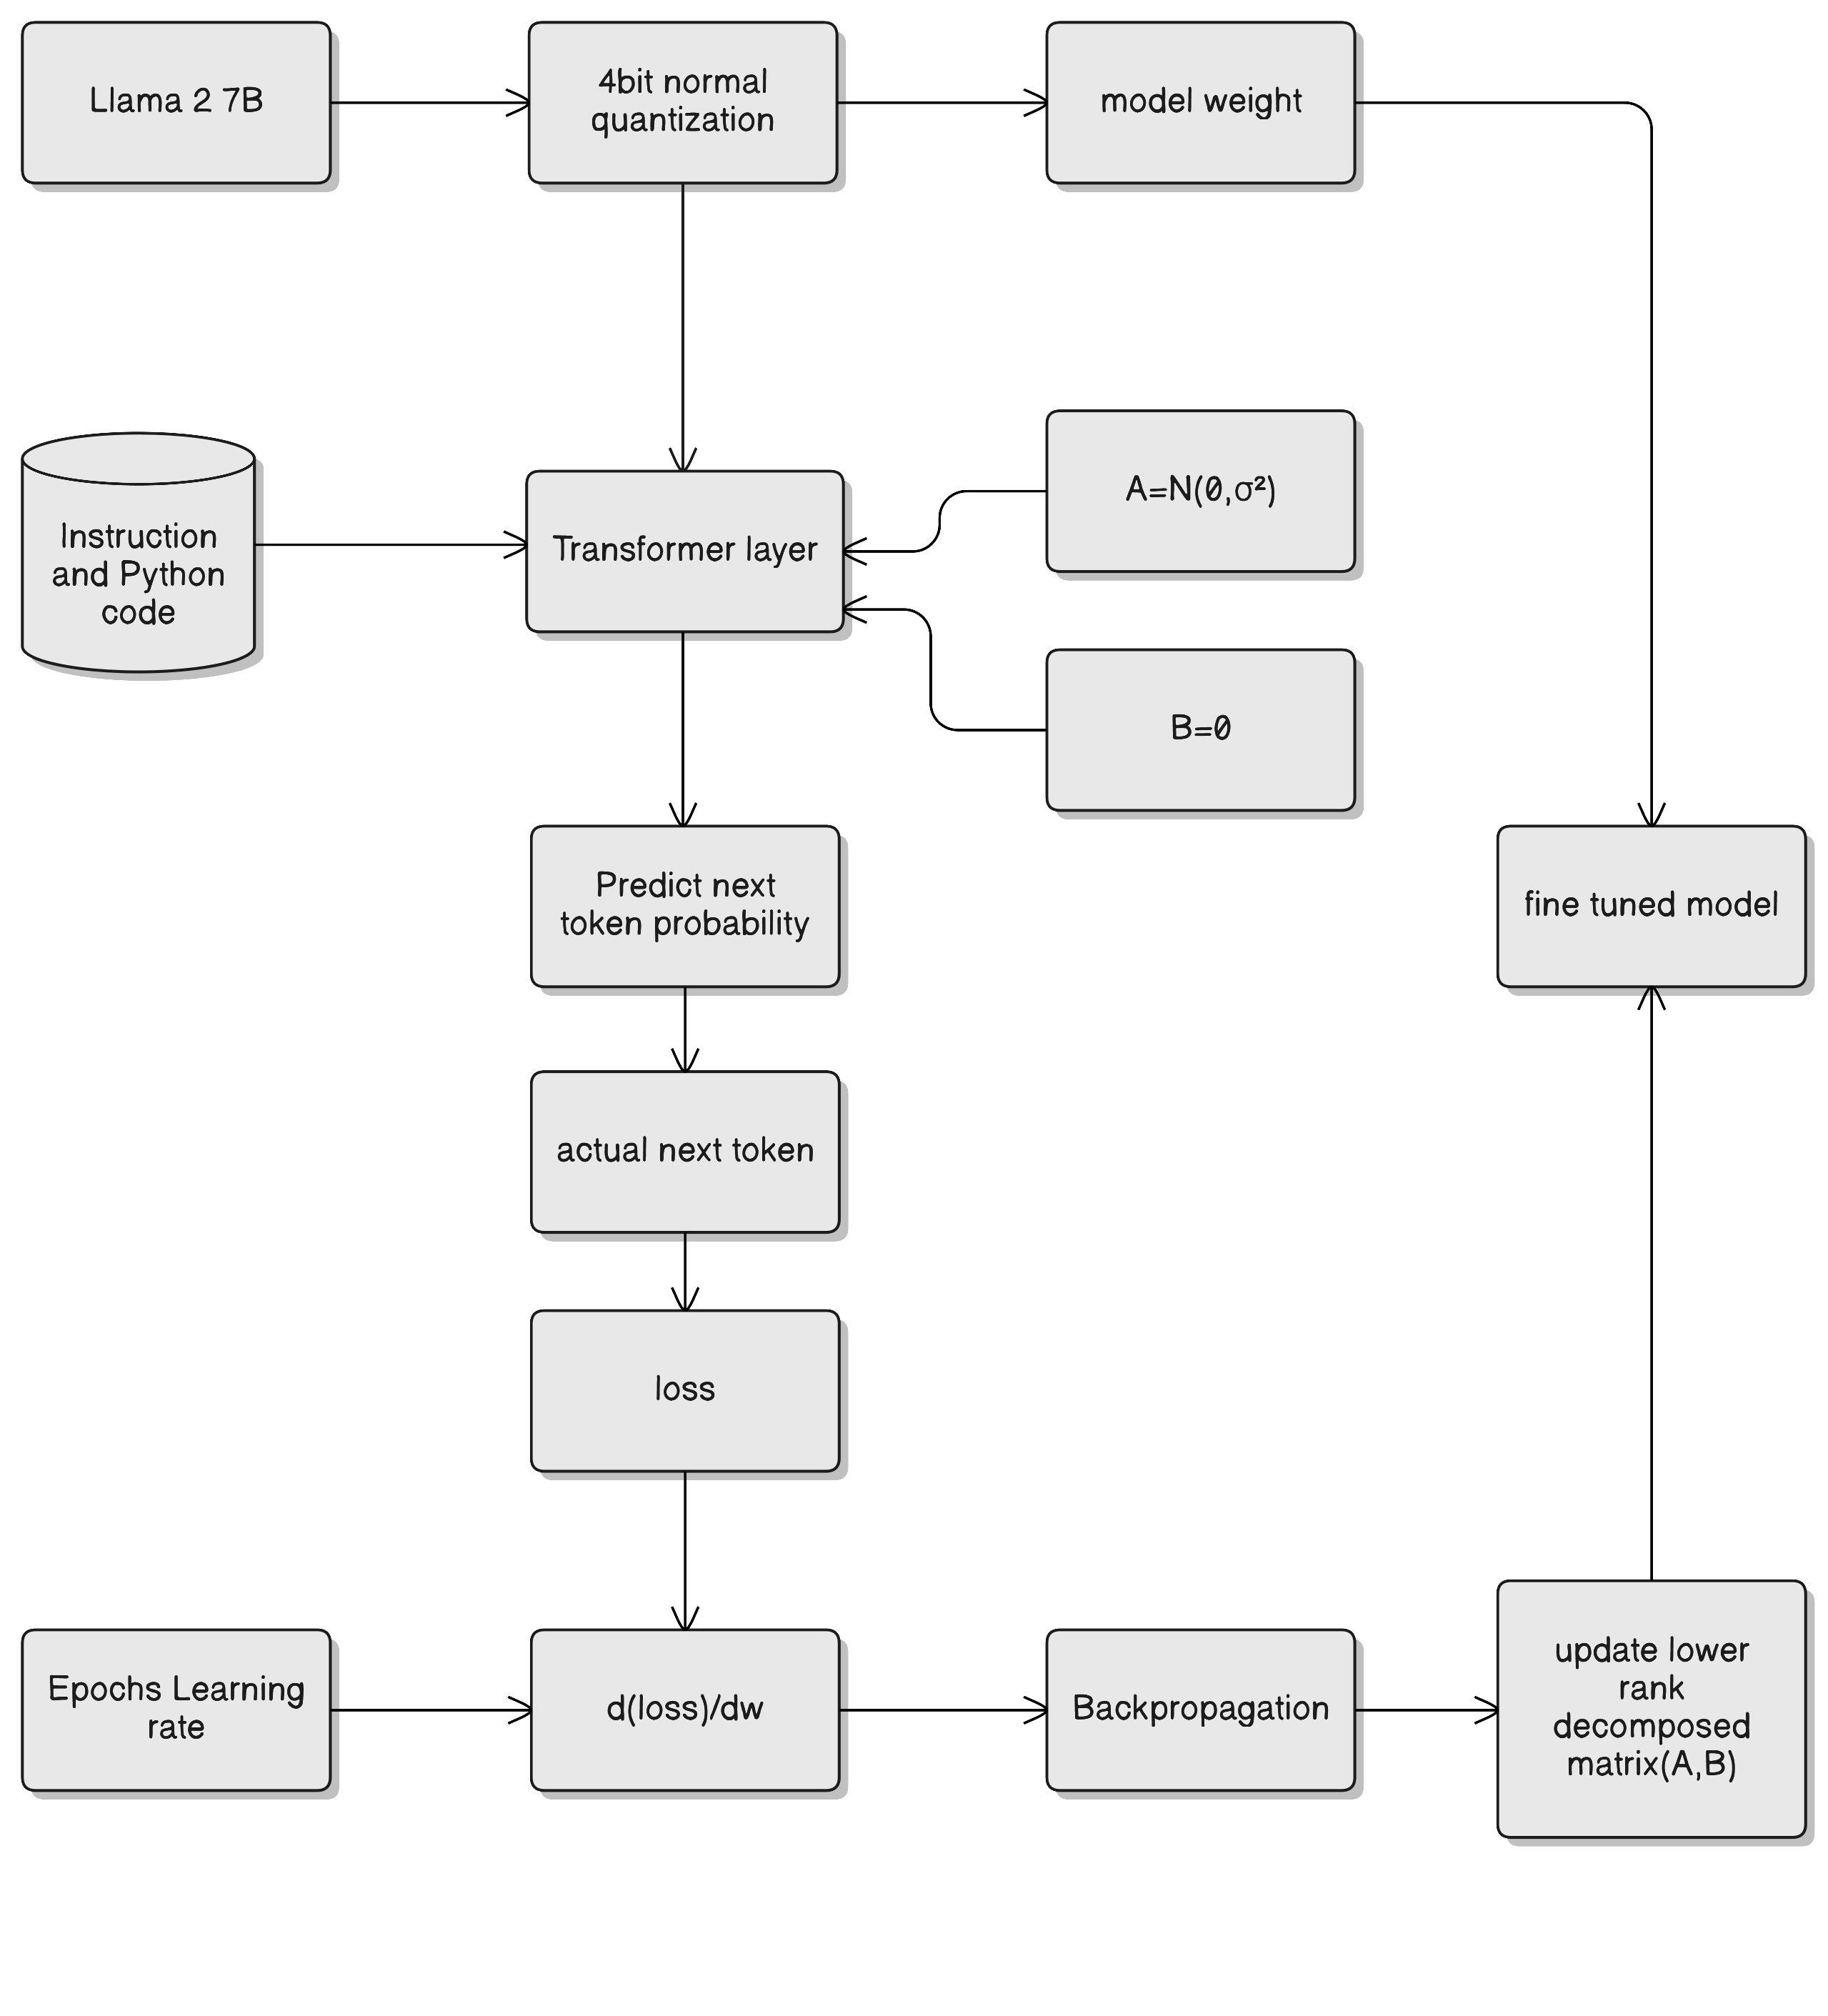
\includegraphics[width=1\linewidth]{flowdiagram.png} 
    % Uncomment when you add the figure
    \caption{Base Model Fine-tuning with QLoRA Adapter Layers}
    \label{figBase Model Finetuning with QLoRA Adapter Layersg}
\end{figure}

Only the adapter matrices are optimized. This allows us to incorporate CoT-augmented samples without increasing memory usage, making training feasible in Google Colab. CoT pairs tend to be longer, but QLoRA’s memory-efficient structure allows handling large token sequences even on limited hardware. The figure \ref{figBase Model Finetuning with QLoRA Adapter Layersg} illustrates the QLoRA fine-tuning process with adapter layers integrated into the transformer blocks.

\end{normaltext}
% ---------------------------------------------------------
\section{Training Setup}
\begin{normaltext}
    \begin{itemize}
        \item \textbf{Platform:} Google Colab
        \item \textbf{Optimizer:} AdamW
        \item \textbf{Hyperparameters:} learning rate, batch size, and epochs tuned using validation loss
        \item \textbf{Regularization:} Dropout applied to adapter layers
        \item \textbf{Early stopping:} Enabled based on validation loss
        \item \textbf{Batching:} Token-based batching, using the maximum number of tokens that fit in GPU memory (typically 8k–32k tokens per batch on Colab)
        \item \textbf{Multiple Session:} If needed, training will be split across multiple Colab sessions with checkpointing
    \end{itemize}


\vspace{18 pt}
\section{Monitoring and Checkpointing} %########write mor here########
The training process will be continuously monitored using WandB, enabling real-time tracking of loss curves, performance metrics, and system resource usage. To ensure recoverability and reproducibility, periodic checkpoints will be saved both locally and to Google Drive throughout training, while the final optimized model will be uploaded to the Hugging Face Hub for easy access and deployment. Randomness across data loading, model initialization, and training operations will be controlled using fixed random seeds, ensuring deterministic and repeatable experiments. Additionally, DVC will be employed to manage and control versions of the fine-tuning datasets, providing a robust and traceable data pipeline that supports reliable experimentation and model iteration.
\end{normaltext}


% ---------------------------------------------------------
\section{Evaluation}
\begin{normaltext}
The fine-tuned model will be compared against the base Llama 2 7B model using two evaluation strategies.
\begin{enumerate}
    \item{\textbf{Functional Correctness (Primary Evaluation)}}

        Generated solutions will be executed in a secure Docker-based sandbox. Each result is classified as

        \begin{itemize}
            \item \textbf{Right} Correct output for all test cases
            \item \textbf{Partial} Runs but fails some test cases
            \item \textbf{Wrong} Crashes or produces incorrect output
        \end{itemize}

        This directly measures true problem-solving ability.

        \item{\textbf{Automatic Similarity Metrics (BLEU, CodeBLEU)}}

        \begin{itemize}
            \item \textbf{BLEU} 
            \\BLEU Evaluates token-level n-gram overlap between generated and reference code \cite{Papineni2002}. The BLEU score is computed using \eqref{eq:bleu}:
            
            \begin{equation}\label{eq:bleu}
            	{BLEU} = \text{BP} \cdot \exp\left(\sum_{n=1}^{N} w_n \log p_n\right)
            \end{equation}
            
            where $p_n$ is the n-gram precision, $w_n$ are uniform weights (typically $w_n = 1/N$), and BP is the brevity penalty is calculated using equation \eqref{eq:bleu_bp}:
            
            \begin{equation}\label{eq:bleu_bp}
            	{BP} = \begin{cases} 
            1 & \text{if } c > r \\
            e^{(1-r/c)} & \text{if } c \leq r
            \end{cases}
            \end{equation}
            The n-gram precision $p_n$ uses clipped counts to avoid rewarding repeated tokens:

            \begin{equation}\label{eq:pn}
            p_{n}=\frac{\sum _{\text{candidate\ sentences}}\sum _{\text{n-gram}\in \text{candidate}}\text{Count}_{\text{clip}}(\text{n-gram})}{\sum _{\text{candidate\ sentences}}\sum _{\text{n-gram}\in \text{candidate}}\text{Count}(\text{n-gram})}
            \end{equation}
            
            where $c$ and $r$ are as defined for BP in \eqref{eq:bleu_bp}; the clipped n-gram precision $p_n$ is given by \eqref{eq:pn}.

            \item \textbf{CodeBLEU} 
            \\CodeBLEU extends BLEU for code generation \cite{Brown2020}, taking into account syntax, data-flow, and semantic correctness. Mathematically, CodeBLEU is a described by
        \eqref{eq:codebleu}:

        \begin{equation}\label{eq:codebleu}
            \text{CodeBLEU} = \alpha \cdot \text{BLEU} + \beta \cdot \text{AST} + \gamma \cdot \text{DFScore} + \delta \cdot \text{SemanticScore}
                        \end{equation}

                        where $\alpha$, $\beta$, $\gamma$, and $\delta$ are weighting parameters that control the contribution of each component. The individual components are computed as:

                        \begin{equation}\label{eq:ast}
                            \text{AST} = \frac{\text{matching\_subtrees}}{\text{total\_subtrees}}
                        \end{equation}

                        \begin{equation}\label{eq:dfscore}
                            \text{DFScore} = \frac{\text{matching\_dataflow\_edges}}{\text{total\_dataflow\_edges}}
                        \end{equation}

                        \begin{equation}\label{eq:semantic}
                            \text{SemanticScore} = \frac{\text{matching\_semantic\_tokens}}{\text{total\_semantic\_tokens}}
                        \end{equation}

                        BLEU token matching, AST syntactic structure, data-flow analysis, and semantic correctness respectively.
                        \end{itemize}

        These are used as supporting quantitative metrics alongside functional evaluation.

    \item{\textbf{Combined Evaluation Insight}}

        By combining functional execution with similarity-based metrics, we ensure that the generated Python code is not only syntactically valid but also meaningful and semantically aligned with correct solutions.
\end{enumerate}

\end{normaltext}